\chapter{適用例}\label{cha:Indication}
本章では、本提案手法を適用した適用例を示す。
本提案手法を適用する帳票画像を、以下の図\ref{fig:indication_original}に示す。

\begin{figure}[t]
    \begin{center}
        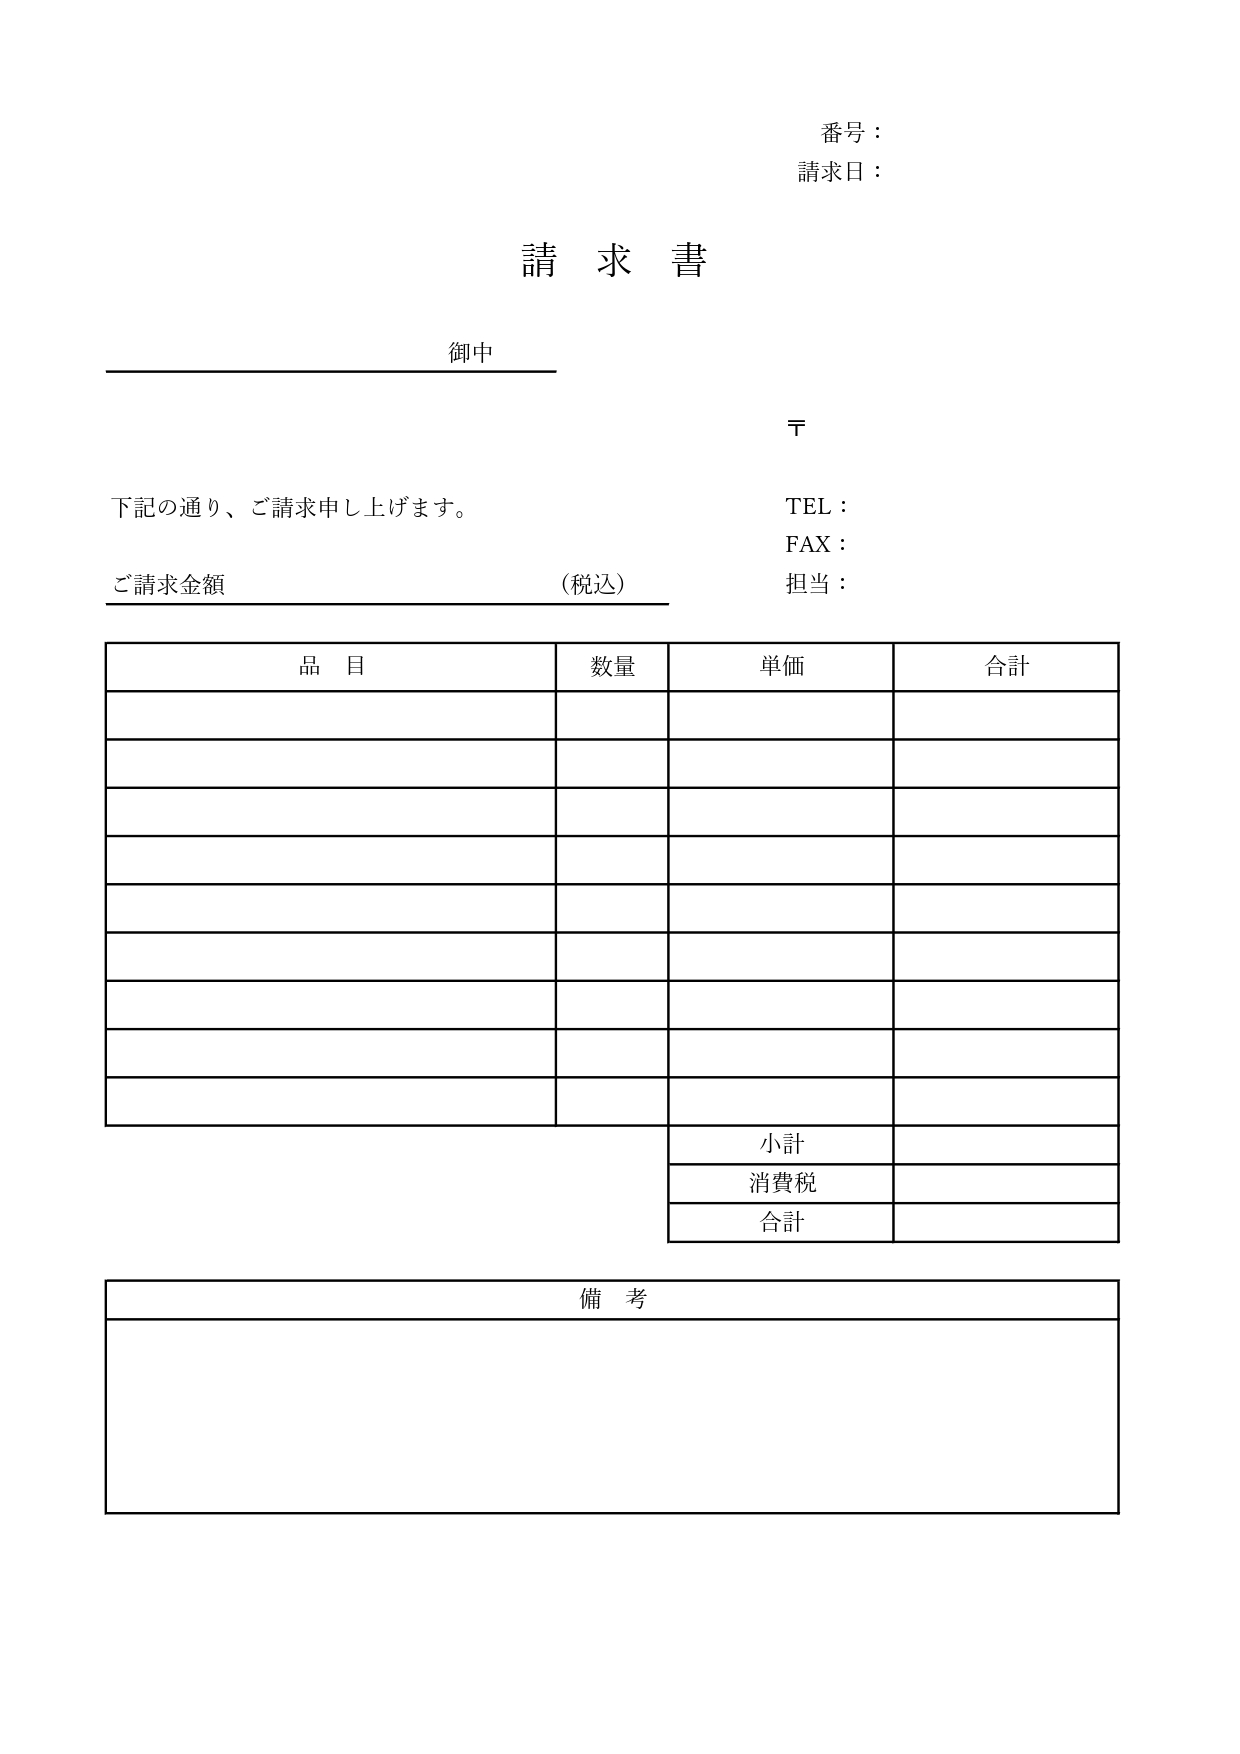
\includegraphics[width=15cm]{image/05-indication/indication_original.jpg}
        \caption{本提案手法を適用する帳票画像}
        \label{fig:indication_original}
    \end{center}
\end{figure}


\section{領域座標取得部の出力結果}\label{sec:result_area_coords_obtainment}
図\ref{fig:indication_original}の帳票画像に対して、矩形領域座標を取得した結果を以下の図に示す。
また、図\ref{fig:indication_original}の帳票画像に対して、下線部領域座標を取得した結果を以下の図に示す。


\begin{figure}[t]
    \begin{center}
        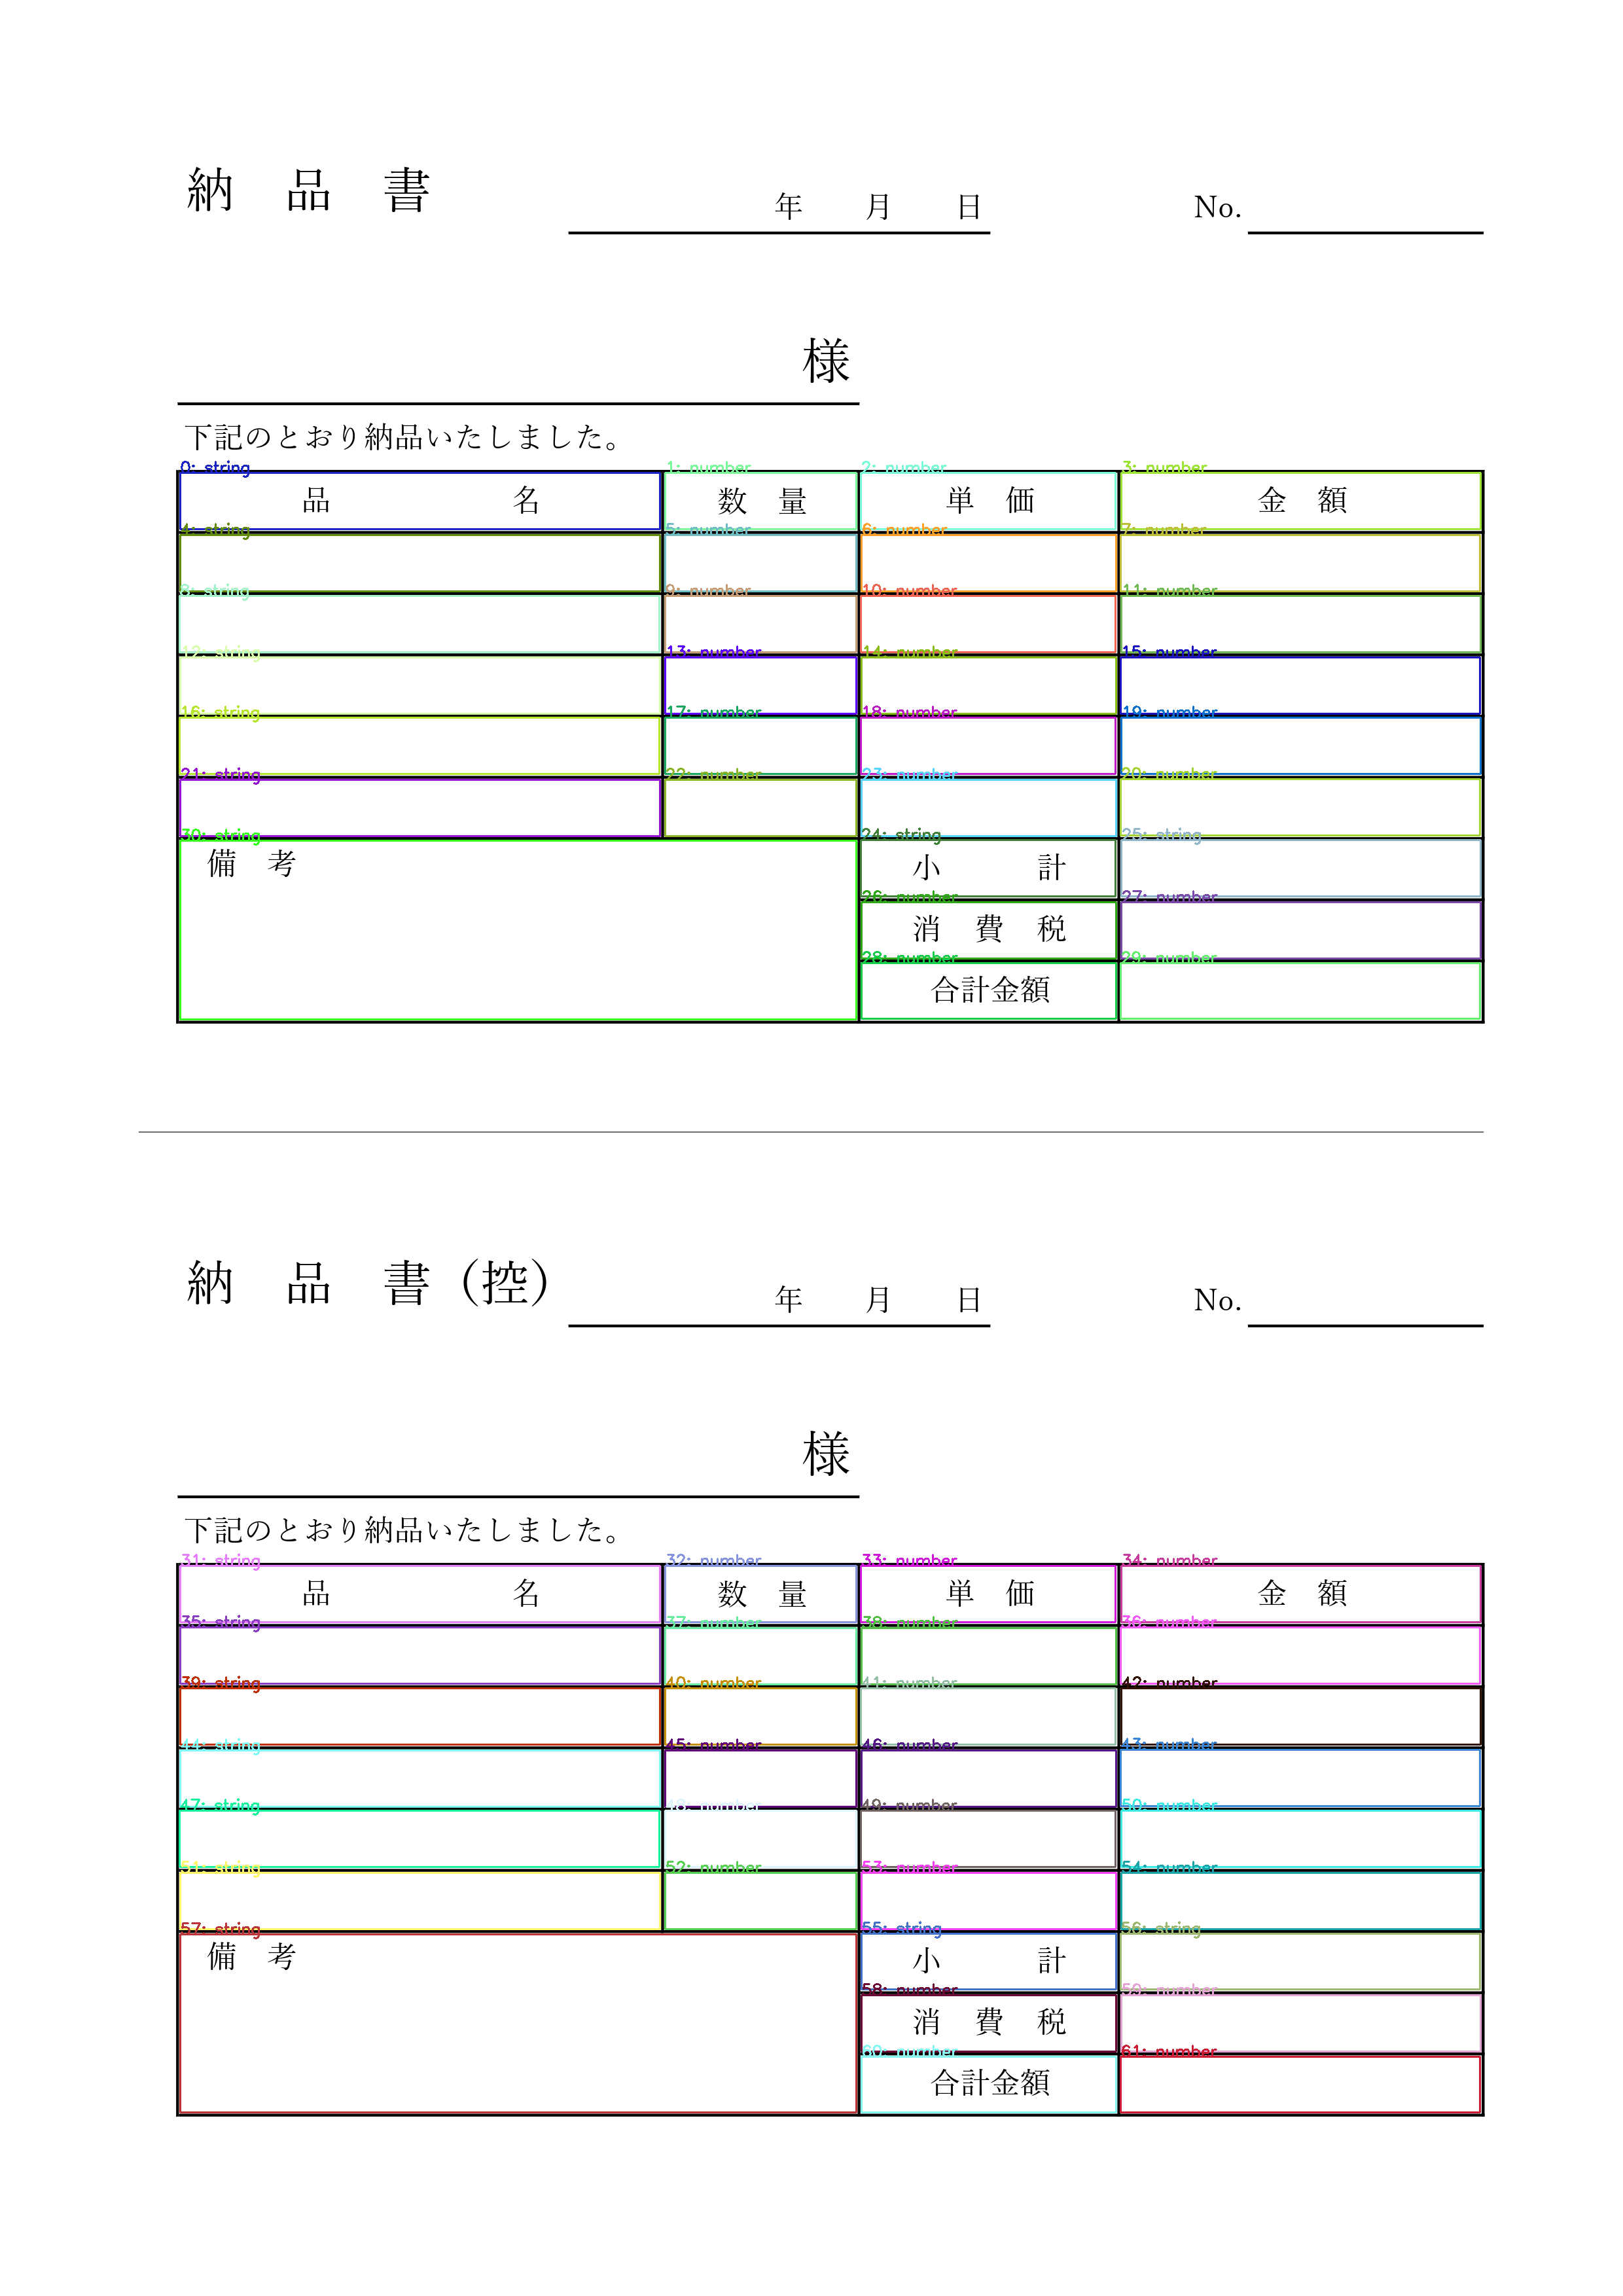
\includegraphics[width=15cm]{image/05-indication/rects_with_label.png}
        \caption{矩形領域座標の取得結果}
        \label{fig:rects_with_label}
    \end{center}
\end{figure}

\begin{figure}[t]
    \begin{center}
        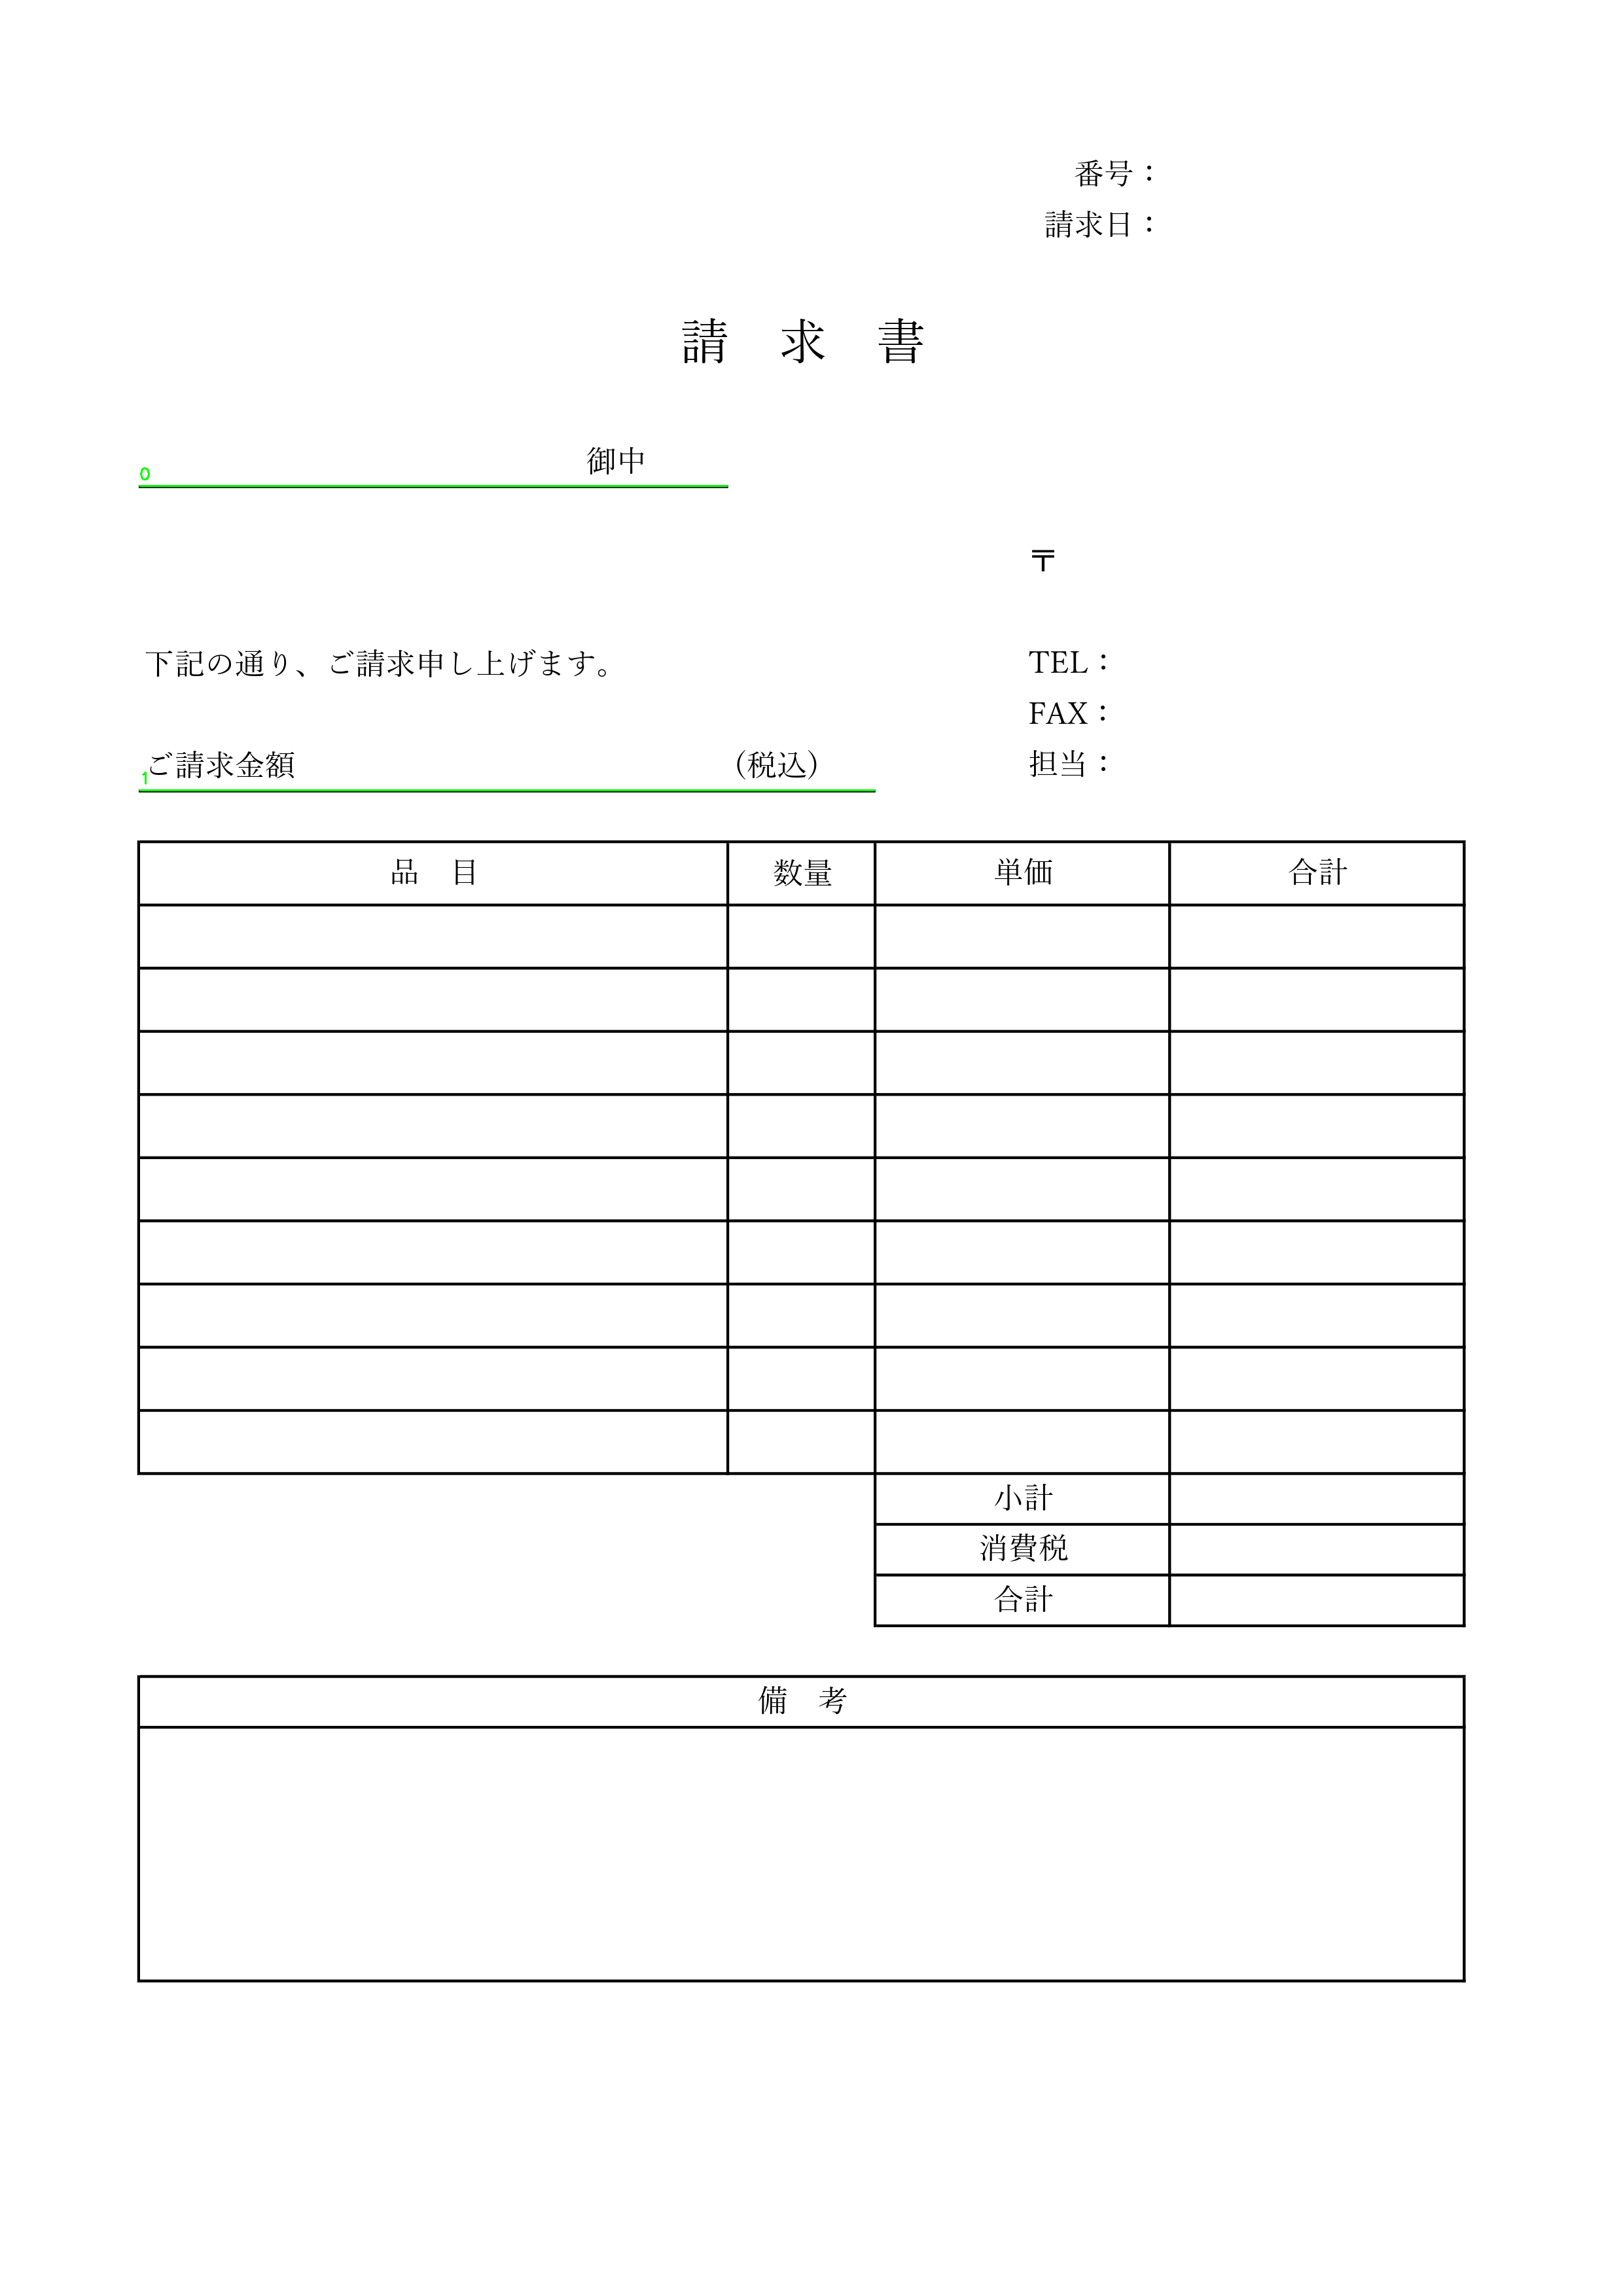
\includegraphics[width=15cm]{image/05-indication/underlines.png}
        \caption{下線部領域座標の出力結果}
        \label{fig:underlines_with_label}
    \end{center}
\end{figure}



\section{文字情報取得部の出力結果}\label{sec:result_OCR}
図\ref{fig:indication_original}の帳票画像に対して、文字情報を取得した結果を以下の図に示す。

\begin{figure}[t]
    \begin{center}
        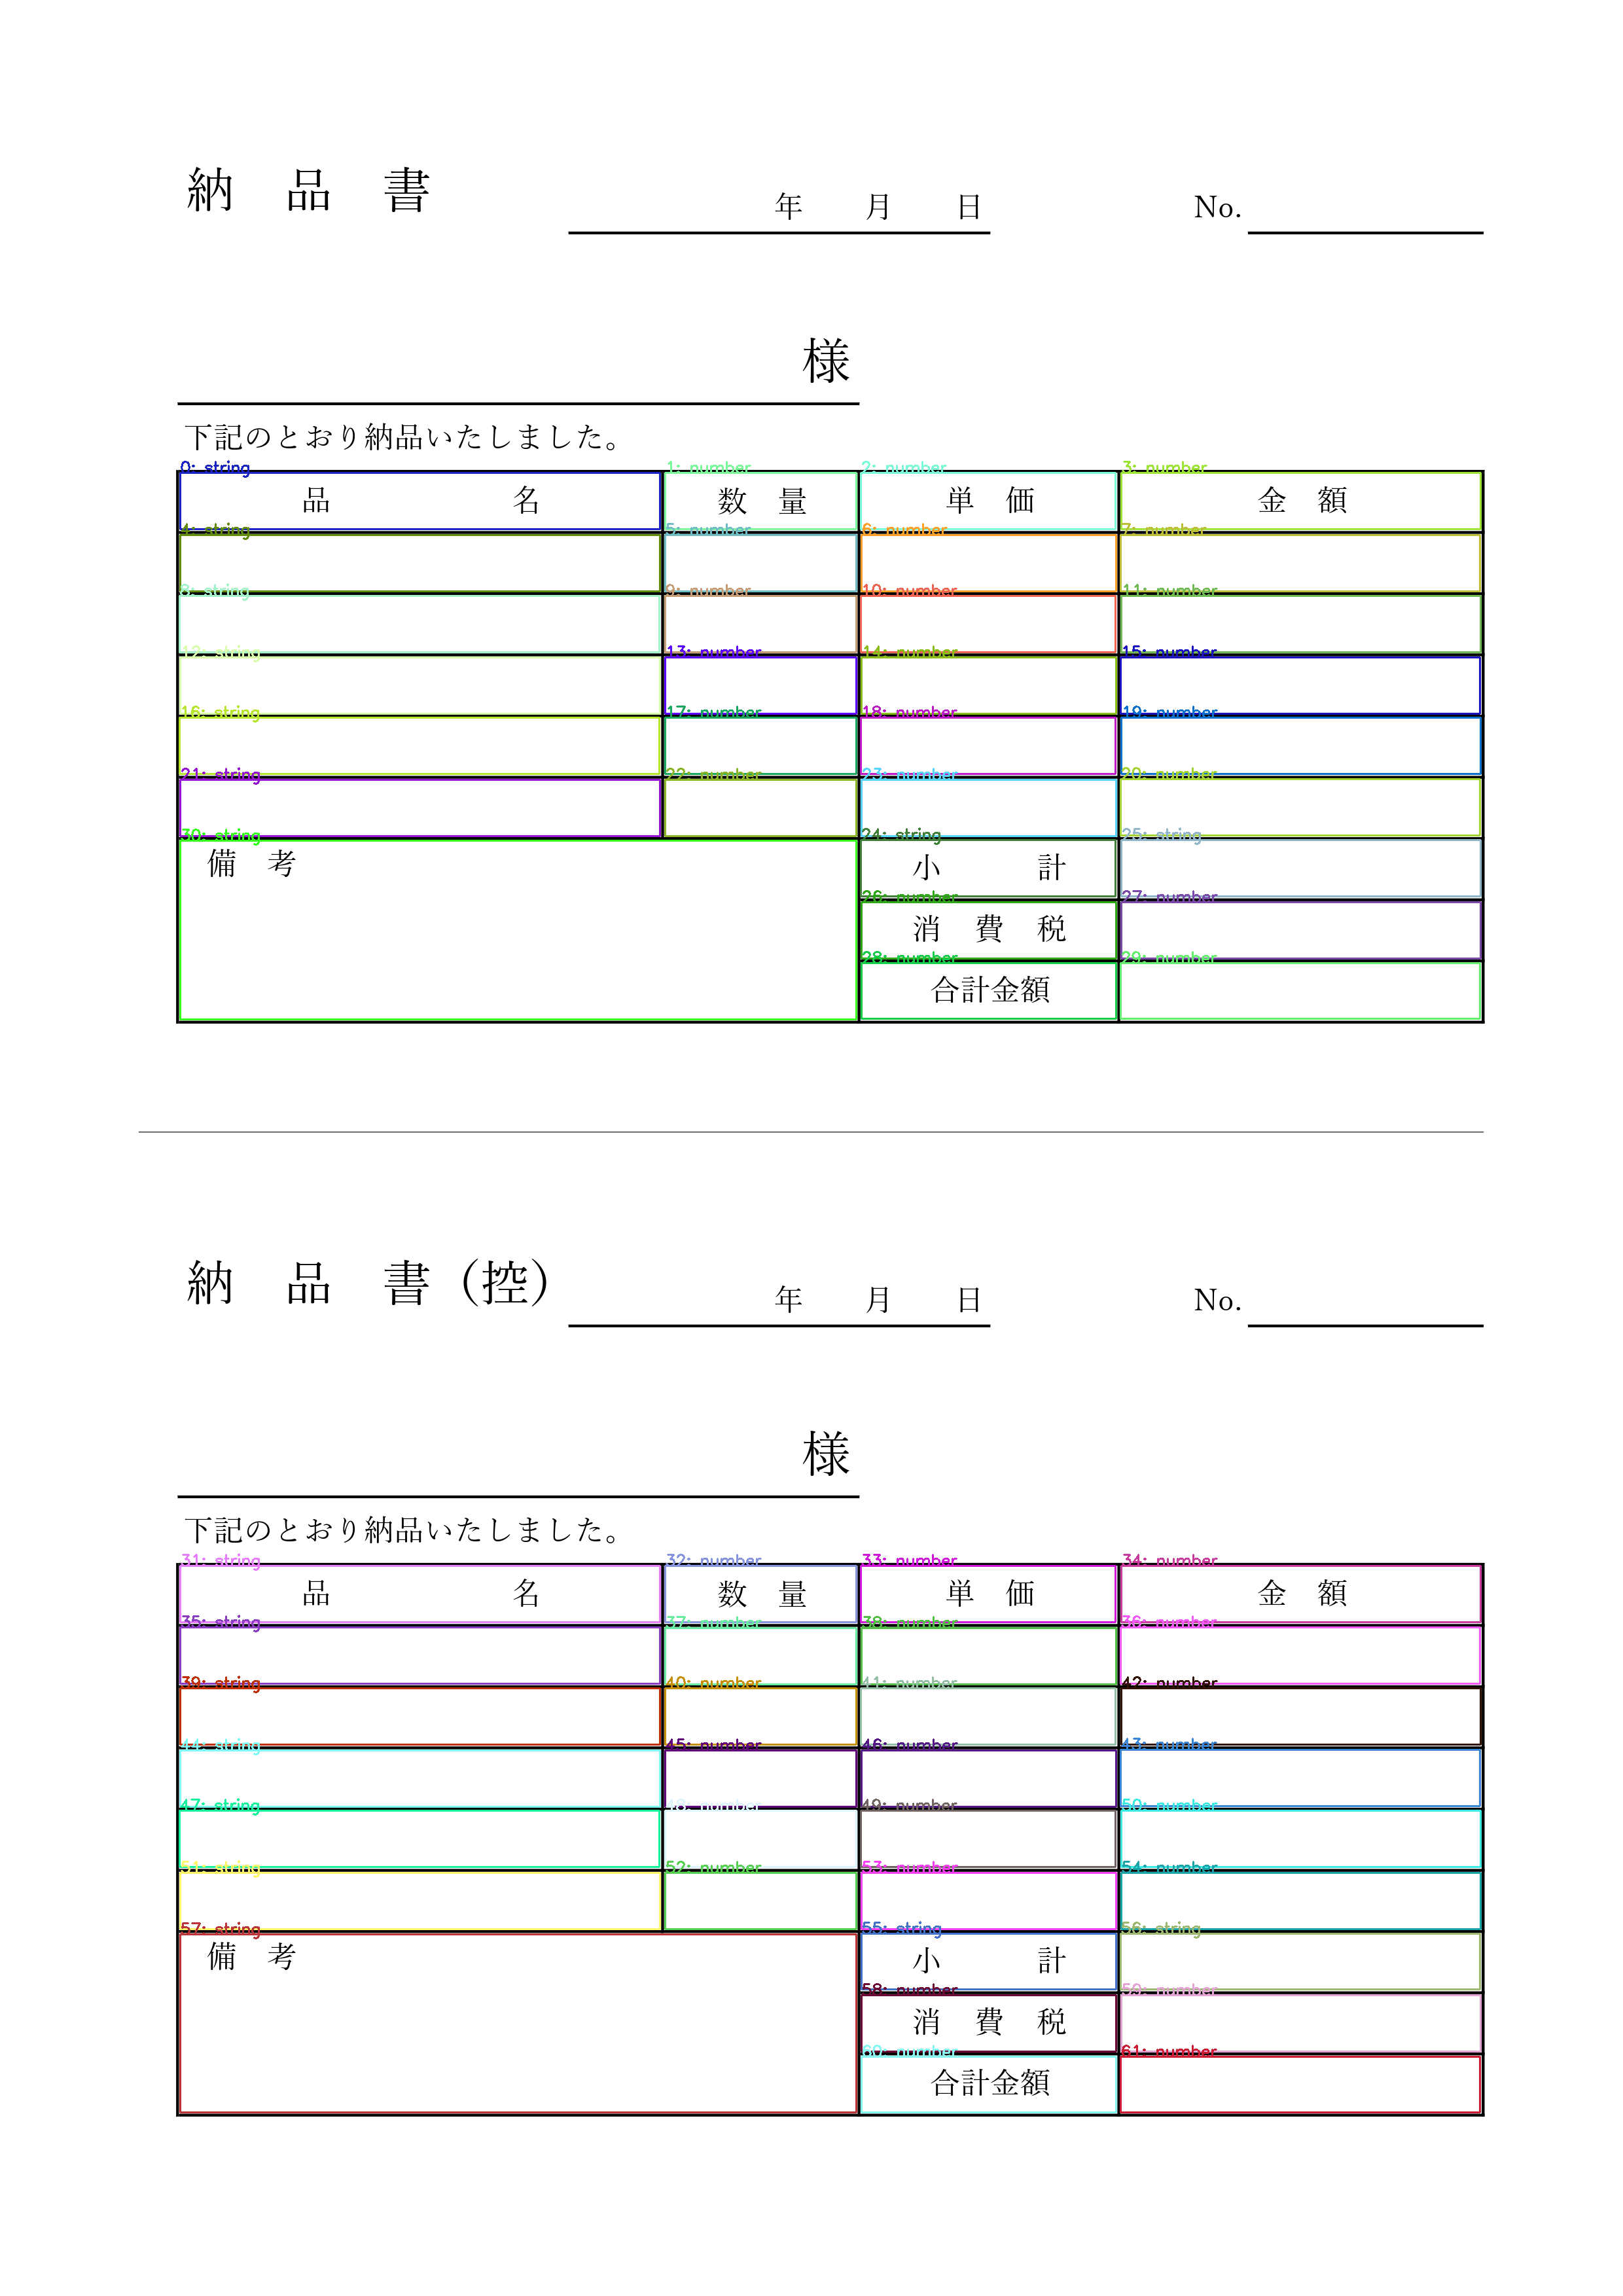
\includegraphics[width=15cm]{image/05-indication/rects_with_label.png}
        \caption{文字情報取得部の出力結果}
        \label{fig:}
    \end{center}
\end{figure}

\section{ラベル付与部の動作結果}\label{sec:result_area_labeling}
図\ref{fig:indication_original}の帳票画像に対して、ラベル付きの矩形領域座標を取得した結果を以下の図に示す。
また、図\ref{fig:indication_original}の帳票画像に対して、ラベル付きの下線部領域座標を取得した結果を以下の図に示す。

\begin{figure}[t]
    \begin{center}
        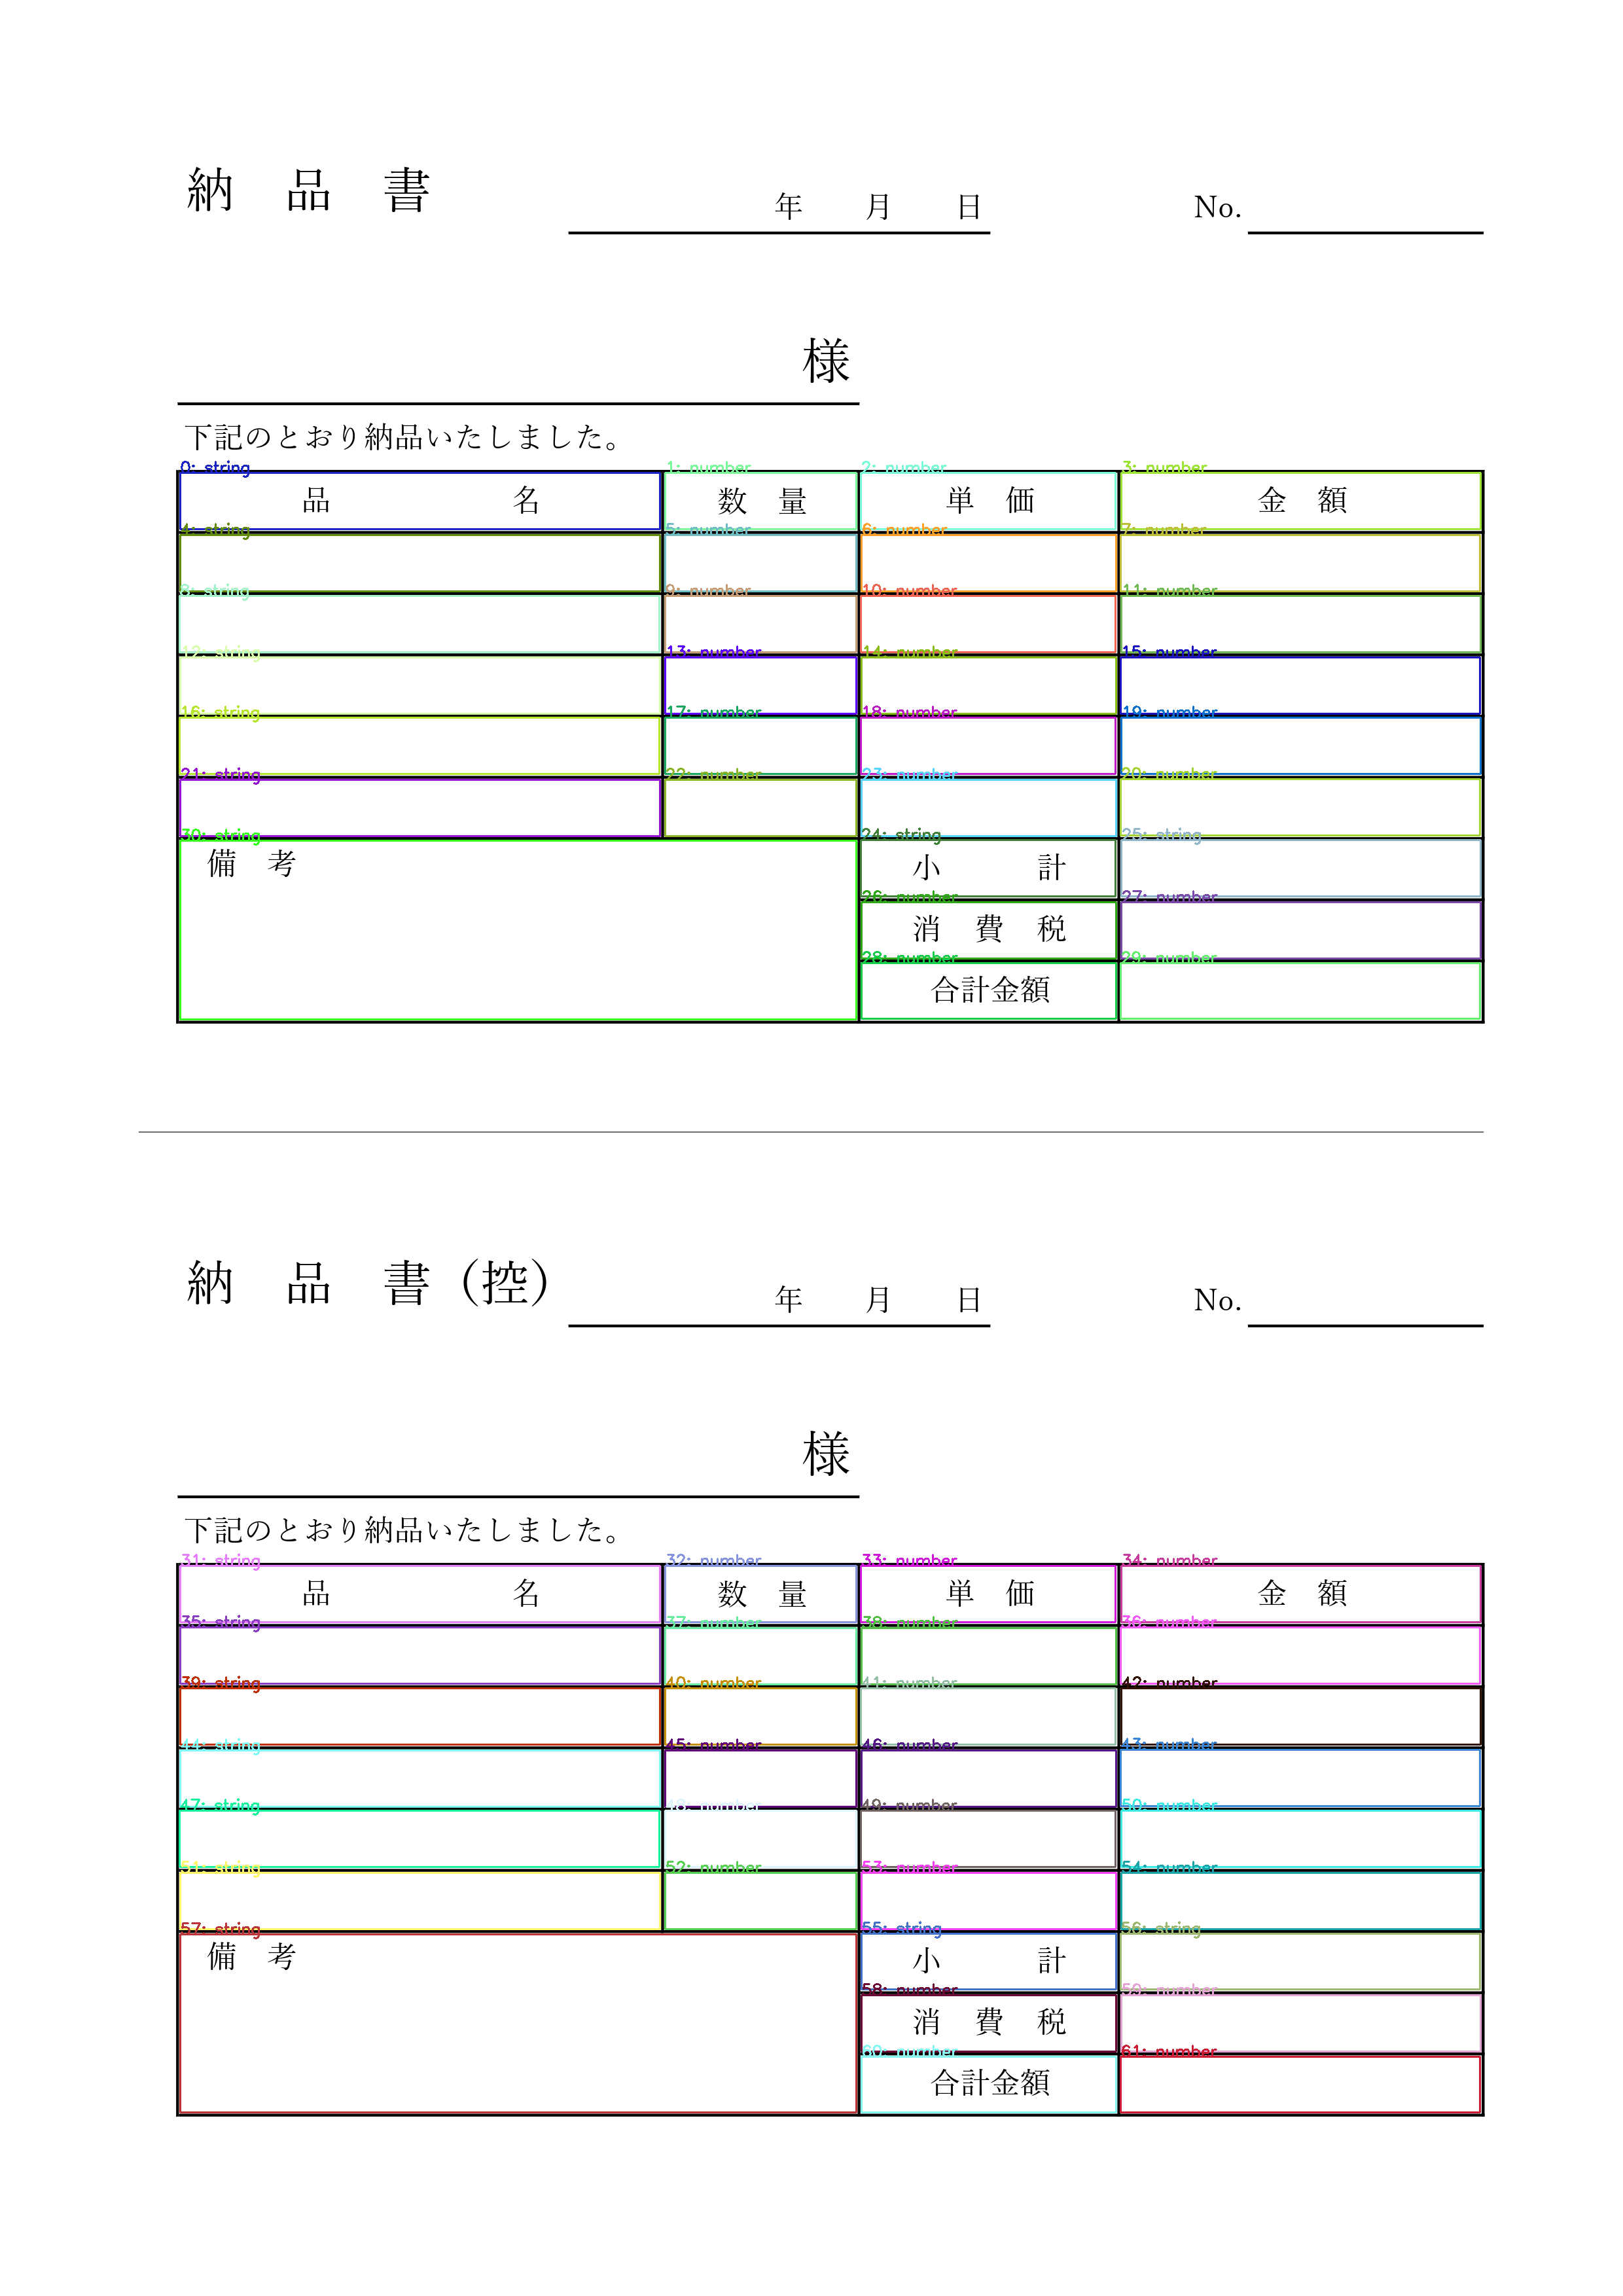
\includegraphics[width=15cm]{image/05-indication/rects_with_label.png}
        \caption{ラベル付き矩形領域座標の取得結果}
        \label{fig:rects_with_label}
    \end{center}
\end{figure}

\begin{figure}[t]
    \begin{center}
        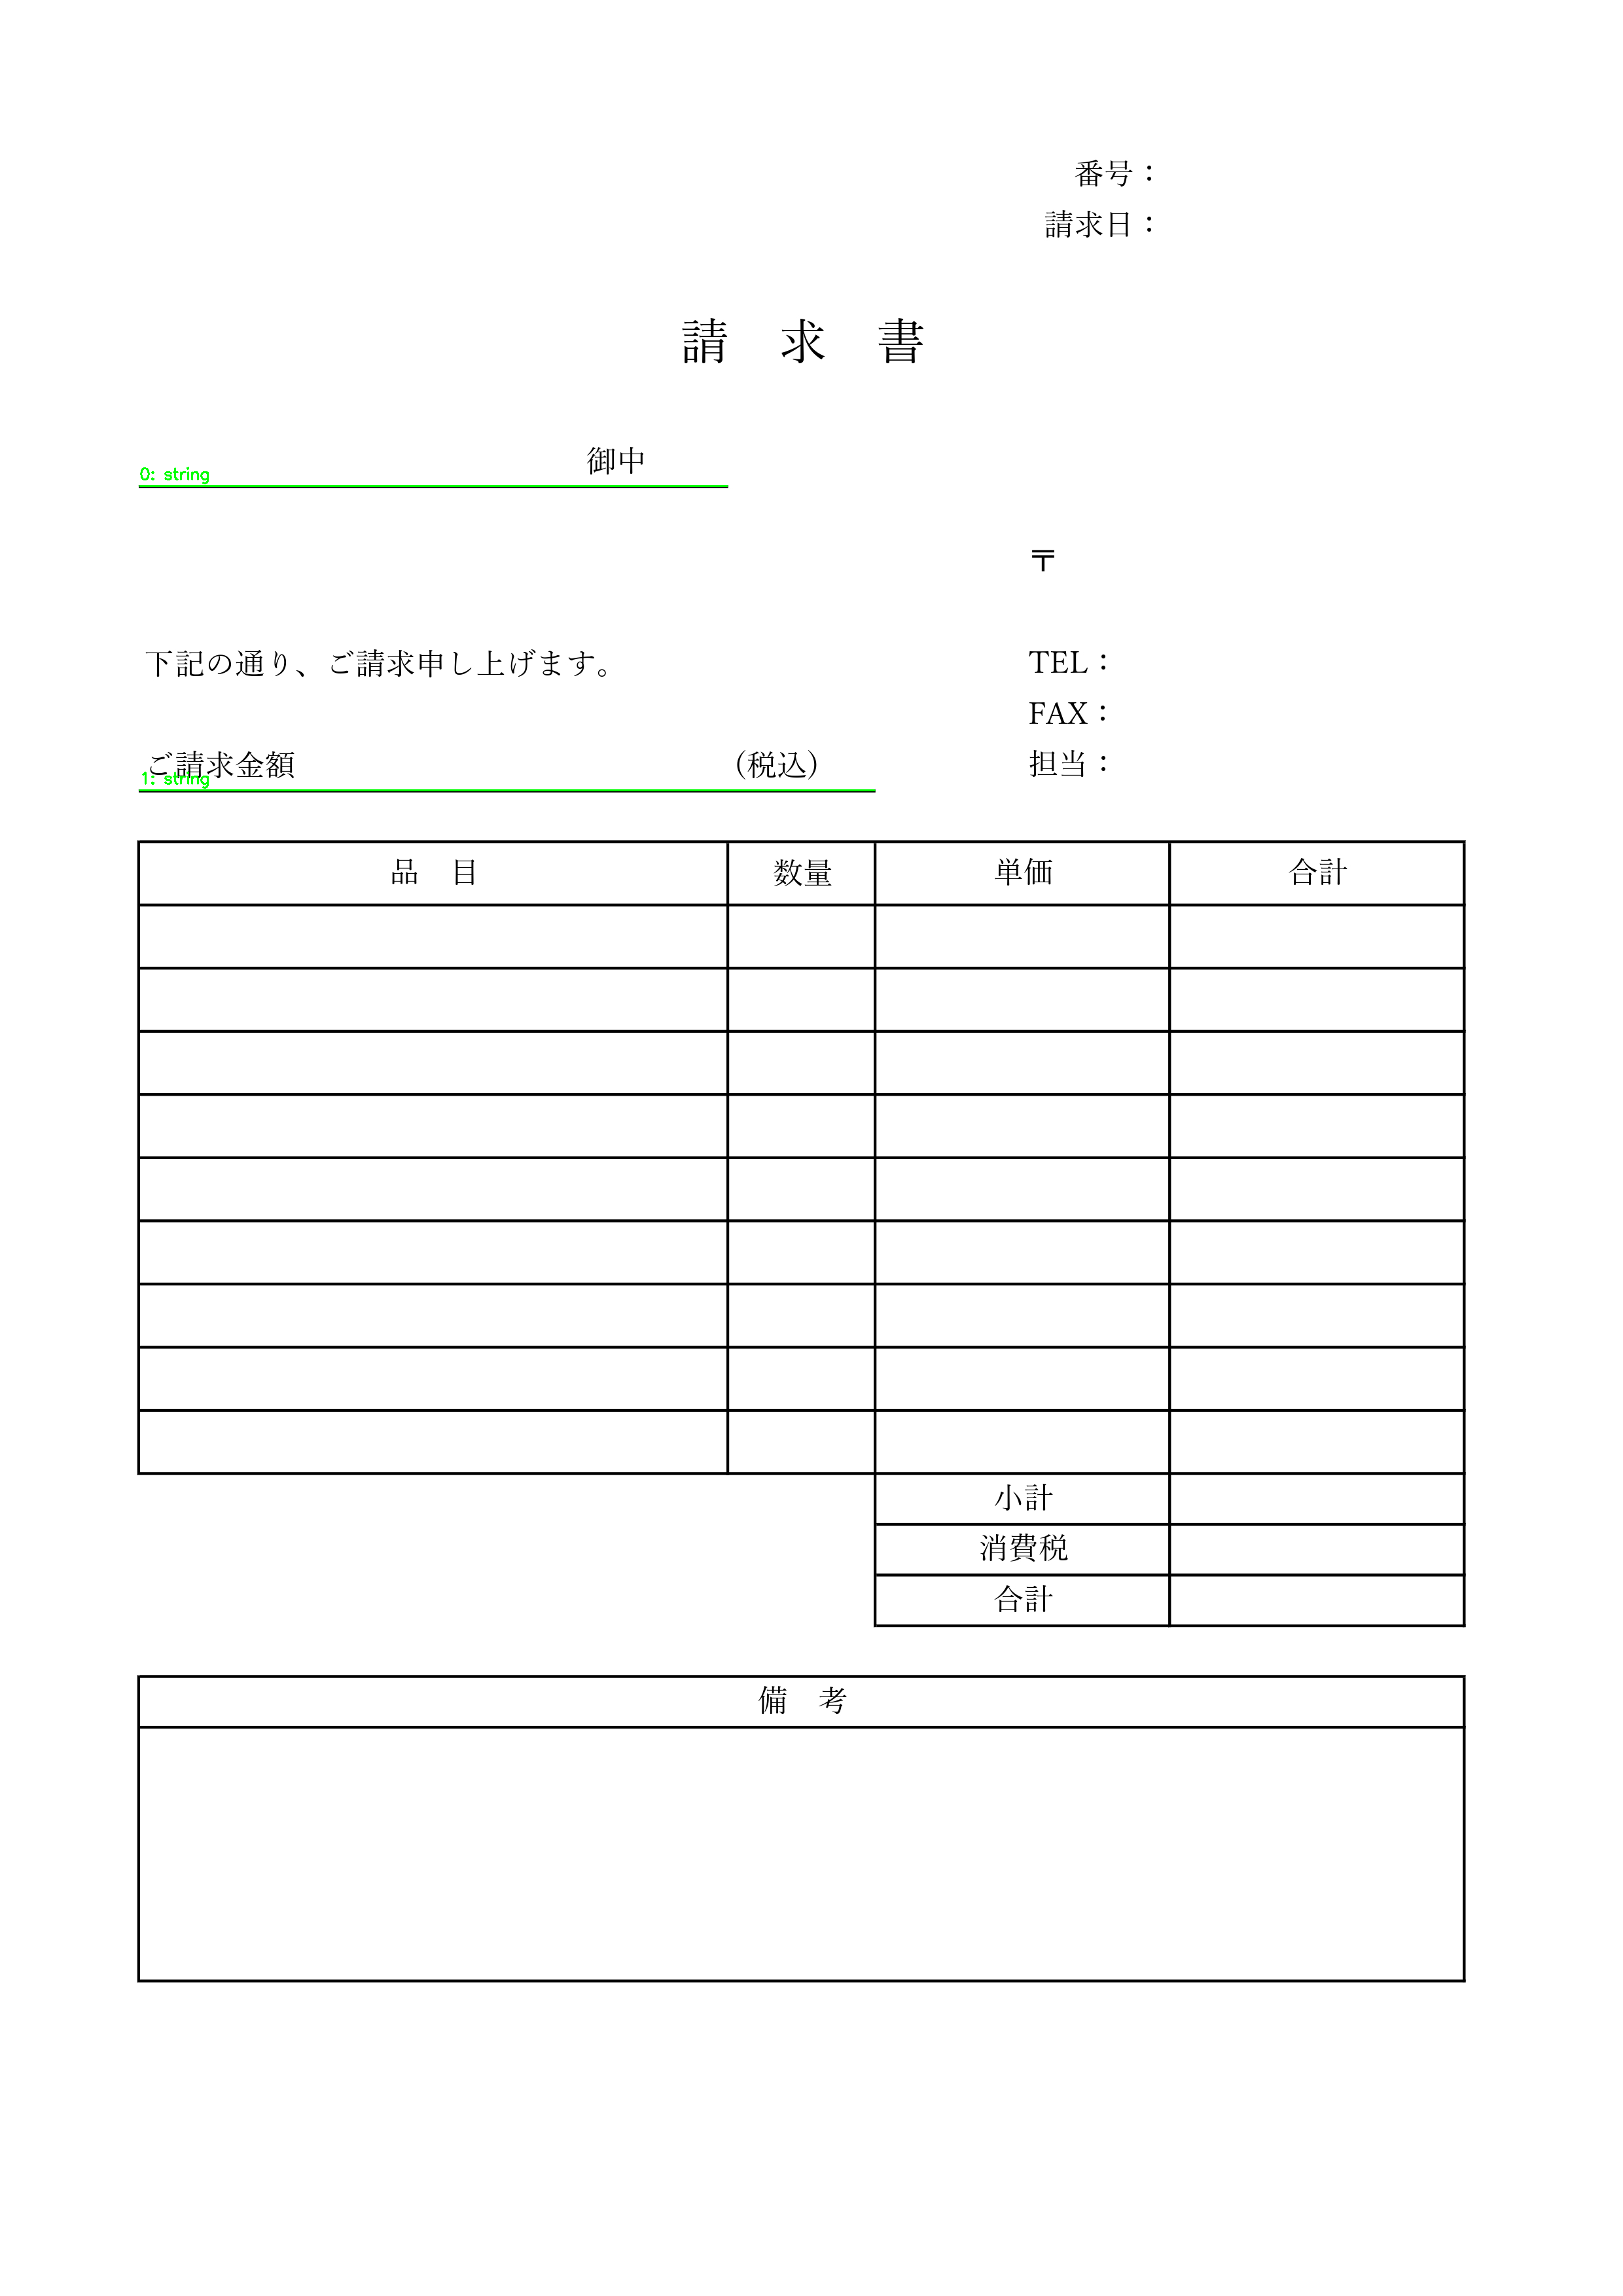
\includegraphics[width=15cm]{image/05-indication/underlines_with_label.png}
        \caption{ラベル付き下線部領域座標の出力結果}
        \label{fig:underlines_with_label}
    \end{center}
\end{figure}